\documentclass[english,floatsintext,man]{apa6}

\usepackage{amssymb,amsmath}
\usepackage{ifxetex,ifluatex}
\usepackage{fixltx2e} % provides \textsubscript
\ifnum 0\ifxetex 1\fi\ifluatex 1\fi=0 % if pdftex
  \usepackage[T1]{fontenc}
  \usepackage[utf8]{inputenc}
\else % if luatex or xelatex
  \ifxetex
    \usepackage{mathspec}
    \usepackage{xltxtra,xunicode}
  \else
    \usepackage{fontspec}
  \fi
  \defaultfontfeatures{Mapping=tex-text,Scale=MatchLowercase}
  \newcommand{\euro}{€}
\fi
% use upquote if available, for straight quotes in verbatim environments
\IfFileExists{upquote.sty}{\usepackage{upquote}}{}
% use microtype if available
\IfFileExists{microtype.sty}{\usepackage{microtype}}{}

% Table formatting
\usepackage{longtable, booktabs}
\usepackage{lscape}
% \usepackage[counterclockwise]{rotating}   % Landscape page setup for large tables
\usepackage{multirow}		% Table styling
\usepackage{tabularx}		% Control Column width
\usepackage[flushleft]{threeparttable}	% Allows for three part tables with a specified notes section
\usepackage{threeparttablex}            % Lets threeparttable work with longtable

% Create new environments so endfloat can handle them
% \newenvironment{ltable}
%   {\begin{landscape}\begin{center}\begin{threeparttable}}
%   {\end{threeparttable}\end{center}\end{landscape}}

\newenvironment{lltable}
  {\begin{landscape}\begin{center}\begin{ThreePartTable}}
  {\end{ThreePartTable}\end{center}\end{landscape}}




% The following enables adjusting longtable caption width to table width
% Solution found at http://golatex.de/longtable-mit-caption-so-breit-wie-die-tabelle-t15767.html
\makeatletter
\newcommand\LastLTentrywidth{1em}
\newlength\longtablewidth
\setlength{\longtablewidth}{1in}
\newcommand\getlongtablewidth{%
 \begingroup
  \ifcsname LT@\roman{LT@tables}\endcsname
  \global\longtablewidth=0pt
  \renewcommand\LT@entry[2]{\global\advance\longtablewidth by ##2\relax\gdef\LastLTentrywidth{##2}}%
  \@nameuse{LT@\roman{LT@tables}}%
  \fi
\endgroup}


  \usepackage{graphicx}
  \makeatletter
  \def\maxwidth{\ifdim\Gin@nat@width>\linewidth\linewidth\else\Gin@nat@width\fi}
  \def\maxheight{\ifdim\Gin@nat@height>\textheight\textheight\else\Gin@nat@height\fi}
  \makeatother
  % Scale images if necessary, so that they will not overflow the page
  % margins by default, and it is still possible to overwrite the defaults
  % using explicit options in \includegraphics[width, height, ...]{}
  \setkeys{Gin}{width=\maxwidth,height=\maxheight,keepaspectratio}
\ifxetex
  \usepackage[setpagesize=false, % page size defined by xetex
              unicode=false, % unicode breaks when used with xetex
              xetex]{hyperref}
\else
  \usepackage[unicode=true]{hyperref}
\fi
\hypersetup{breaklinks=true,
            pdfauthor={},
            pdftitle={Evolution of Statistical Software and Quantitative Methods in Educational Research},
            colorlinks=true,
            citecolor=blue,
            urlcolor=blue,
            linkcolor=blue,
            pdfborder={0 0 0}}
\urlstyle{same}  % don't use monospace font for urls

\setlength{\parindent}{0pt}
%\setlength{\parskip}{0pt plus 0pt minus 0pt}

\setlength{\emergencystretch}{3em}  % prevent overfull lines

\ifxetex
  \usepackage{polyglossia}
  \setmainlanguage{}
\else
  \usepackage[english]{babel}
\fi

% Manuscript styling
\captionsetup{font=singlespacing,justification=justified}
\usepackage{csquotes}
\usepackage{upgreek}



\usepackage{tikz} % Variable definition to generate author note

% fix for \tightlist problem in pandoc 1.14
\providecommand{\tightlist}{%
  \setlength{\itemsep}{0pt}\setlength{\parskip}{0pt}}

% Essential manuscript parts
  \title{Evolution of Statistical Software and Quantitative Methods in
Educational Research}

  \shorttitle{Evolution Software and Methods}


  \author{Brandon LeBeau\textsuperscript{1}~\& Ariel Aloe\textsuperscript{1}}

  \def\affdep{{"", ""}}%
  \def\affcity{{"", ""}}%

  \affiliation{
    \vspace{0.5cm}
          \textsuperscript{1} University of Iowa  }

 % If no author_note is defined give only author information if available
    \authornote{
    \newcounter{author}
                      Correspondence concerning this article should be addressed to Brandon LeBeau, Psychological and Quantitative Foundations, University of Iowa, Iowa
City, IA 52245. E-mail: \href{mailto:brandon-lebeau@uiowa.edu}{\nolinkurl{brandon-lebeau@uiowa.edu}}
                          }
  

  \abstract{Statistical software is the enabling tool of quantitative research
studies and the availability and use of the software can greatly shape
which methods are used by researchers. Software that is more accessible
is likely to have more users and the methods implemented within the
software limits the methods accessible to researchers. Open source
software, (e.g.~R), has reduced these barriers by making cutting edge
statistical methods available to researchers through add-on packages. In
addition, the idea of reproducible analyses has grown significantly
within the statistics and medicine disciplines. This paper aims to
explore the evolution of statistical software within educational
research using a research synthesis to establish the state of affairs.}
  \keywords{Research Synthesis, Statistical Software, Quantitative Methods \\

    
  }





\usepackage{amsthm}
\newtheorem{theorem}{Theorem}
\newtheorem{lemma}{Lemma}
\theoremstyle{definition}
\newtheorem{definition}{Definition}
\newtheorem{corollary}{Corollary}
\newtheorem{proposition}{Proposition}
\theoremstyle{definition}
\newtheorem{example}{Example}
\theoremstyle{remark}
\newtheorem*{remark}{Remark}
\begin{document}

\maketitle

\setcounter{secnumdepth}{0}



\section{Objectives}\label{objectives}

The purpose of this paper is to explore the evolution (or lack thereof)
of statistical software usage over time in education. As this usage is
likely tied closely to the methods they are employed, the interaction
between software usage and quantitative research methods will also be
explored. Research synthesis methods will be used to explore these
trends over time in published educational research journals.

\section{Theoretical Framework}\label{theoretical-framework}

Statistical software is the enabling tool to performing applied data
analysis. Statistical methods that are implemented within software will
increase their usage (particularly if the software is also
user-friendly) by applied analysts and are likely taught more frequently
in methodology courses at universities. However, the user-friendly
nature of software (i.e.~point and click graphical interfaces, ability
to manipulate data by hand) also can severely limit the ability for
research to be reproducible; a recent topic of intense discussion in
biostatistics, medicine, and pyschology (Asendorpf et al., 2013;
Ioannidis, 2014; Iqbal, Wallach, Khoury, Schully, \& Ioannidis, 2016;
Roger D. Peng, 2009; Roger D Peng, 2011; Stodden, 2012). The
reproducibility crisis has pointed the finger at statistical software
more directly with a strong push in some disciplines for analyses to be
script based and posted with the published journal article, often
described as the gold standard.

This idea of reproducibility has not seemed to fully enter the
educational research domain. SPSS is likely the most common statistical
software program used in educational research. Although SPSS has many
common and advanced statistical techniques and it is possible to have a
reproducible analysis, the default behavior within this program is often
not script based and can create bad habits (i.e.~editing raw data
directly in the gui interface, running analyses without saving a script,
etc.). Statistical software that is primarily command line, programs
such as R, Python, or SAS, offer easier reproducible frameworks as all
data manipulations or analyses are saved in scripts that can be re-ran
in the future. A data script can be thought of as a cockpit flight
recorder in which every single step that was done to the original data
going from data collection to final tables and figures was script based.
Under a reproducible framework, the raw data are never altered directly,
they should always be altered programmatically through a script. This
keeps a log of the data manipulations that happened in the data analysis
cycle. For example, R has packages that aid in the ability to create
living data documents that contain text and analysis code within a
single document (see Allaire et al., 2017; Xie, 2015, 2017).

The reproducible analysis framework has many advantages, including a
transparent analysis process that could be validated by others or even
simply the ability to investigate the data analysis completed months or
years previously. Unfortunately, the current academic research framework
has many barriers that limit the reproducibility. First, applied
researchers may not be users of primarily command line or script based
statistical software. This limits the ability to create a reproducible
framework from the start. Secondly, researchers are not incentivized to
conduct an analysis in a reproducible framework. Namely, the publish or
perish aspect of academic research limits the sharing of statistical
code partly due to the increased chance of criticism upon evaluation of
the code used for the analysis. Finally, many journals and even the
American Psychological Association (APA) publication manual (American
Psychological Association, 2010) states that common software or
programming languages need not be cited. This could even be interpretted
by some as not needing to mention. Unfortunately, if the software used
for a data analysis is not reported, the ability to recreate the
analysis drops even more due to differences in estimation, handling of
missing data, or other software specific settings.

This paper aims to explore the state of affairs in statistical software
usage in education. Particular attention will be made to which software
is currently being used in published educational research as well as how
this has changed over the last twenty years. Secondly, this paper also
aims to explore how frequently open-source software tools are used and
to explore evidence of reproducible analysis framework being
implemented. These aims will be explored using research synthesis
methods.

\subsection{Research Questions}\label{research-questions}

\begin{enumerate}
\def\labelenumi{\arabic{enumi}.}
\tightlist
\item
  To what extent has the statistical software usage shifted over time in
  published analyses?

  \begin{itemize}
  \tightlist
  \item
    If there is evidence of a shift, is there evidence this shift
    differs based on quantitative method or journal?
  \end{itemize}
\item
  To what extent are published analyses citing statistical software?

  \begin{itemize}
  \tightlist
  \item
    Has this changed over time and across journals?
  \end{itemize}
\item
  To what extent are open-source software tools used?

  \begin{itemize}
  \tightlist
  \item
    Is there evidence of reproducible analyses being employed?
  \end{itemize}
\end{enumerate}

\section{Methods}\label{methods}

Research synthesis methods (Cooper, 2016) will be used to explore the
evolution of statistical software and quantitative methods in
educational research. More specifically, the statistical software used
for the analysis will be coded in additional to the specific
quantitative methods (i.e.~linear regression, hierarchical linear model,
etc.). Additional meta data will also be coded including, journal,
article title, author information, article keywords, year published, and
any mention of supplementary materials. This information will be used to
explore descriptive trends in the data over time, by journals, and
methods.

The research synthesis will gather data from a handful of education
journals that primarily publish empirical data analysis. The search will
not include journals that the primary focus is methodological, the use
of software in these journals would likely be a different population
than those that are data analytic in nature. Therefore the following
journals were selected to be searched from 1995 onward:

\begin{itemize}
\tightlist
\item
  American Educational Research Journal (AERJ)
\item
  Educational Researcher (ER)
\item
  Educational Evaluation and Policy Analysis (EEPA)
\item
  Higher Education (HE)
\item
  Journal of Educational Psychology (JEP)
\item
  Journal of Experimental Education (JEE)
\item
  Journal of Teacher Education (JTE)
\item
  Journal for Research in Mathematics Education (JRME)
\item
  Sociology of Education (SE)
\end{itemize}

\section{Data and Software}\label{data-and-software}

All journal articles published between 1995 through 2016 will be
organized into EndNote. Within EndNote, the find pdf feature will be
used to gather the published documents from each journal. This pdf
database will then be searched using the \emph{pdfsearch} R package
(LeBeau, 2016, R Core Team (2017)). This package allows for keyword
searching directly within pdf documents. This will be the primary data
collection method. The software keywords searched for can be seen in
Table \ref{tab:searchwords}. Table \ref{tab:searchwords} also shows
keywords to be used to search for statistical models and estimation
methods.

\begin{longtable}[]{@{}ll@{}}
\caption{\label{tab:searchwords} Search keywords used in search of published
journal documents}\tabularnewline
\toprule
\begin{minipage}[b]{0.21\columnwidth}\raggedright\strut
Search\strut
\end{minipage} & \begin{minipage}[b]{0.38\columnwidth}\raggedright\strut
Keywords\strut
\end{minipage}\tabularnewline
\midrule
\endfirsthead
\toprule
\begin{minipage}[b]{0.21\columnwidth}\raggedright\strut
Search\strut
\end{minipage} & \begin{minipage}[b]{0.38\columnwidth}\raggedright\strut
Keywords\strut
\end{minipage}\tabularnewline
\midrule
\endhead
\begin{minipage}[t]{0.21\columnwidth}\raggedright\strut
Software\strut
\end{minipage} & \begin{minipage}[t]{0.38\columnwidth}\raggedright\strut
\enquote{SPSS Statistics}, \enquote{SPSS Modeler}, \enquote{SPSS},
\enquote{R}, \enquote{R-project}, \enquote{R project}, \enquote{SAS},
\enquote{JMP}, \enquote{STATA}, \enquote{MATLAB}, \enquote{Statistica},
\enquote{Statsoft}, \enquote{Java}, \enquote{Hadoop}, \enquote{Python} ,
\enquote{Minitab}, \enquote{Systat}, \enquote{Tableau}, \enquote{Scala},
\enquote{Julia}, \enquote{Azure Machine Learning}, \enquote{Mplus},
\enquote{LISREL}, \enquote{AMOS}, \enquote{HLM{[}0-9{]}}, \enquote{HLM
{[}0-9{]}}\strut
\end{minipage}\tabularnewline
\begin{minipage}[t]{0.21\columnwidth}\raggedright\strut
Statistical Models\strut
\end{minipage} & \begin{minipage}[t]{0.38\columnwidth}\raggedright\strut
Regression, Hierarchical Linear Model (HLM), Linear Mixed Model (LMM),
Multilevel Model, Analysis of Variance (ANOVA), Structural Equation
Modeling (SEM)\strut
\end{minipage}\tabularnewline
\begin{minipage}[t]{0.21\columnwidth}\raggedright\strut
Estimation\strut
\end{minipage} & \begin{minipage}[t]{0.38\columnwidth}\raggedright\strut
Maximum Likelihood, bayesian,\strut
\end{minipage}\tabularnewline
\bottomrule
\end{longtable}

A handful of articles will be randomly selected to be coded manually by
reading the document to evaluate the accuracy of coding from the
\emph{pdfsearch} package.

\section{Initial Results}\label{initial-results}

Currently, published journal articles between the year 2000 and 2014 for
AERJ, EEPA, and JEE have been obtained and the software keyword search
has been performed with the \emph{pdfsearch} package. Table
\ref{tab:setup} reports the number of unique published articles for each
journal that contained at least one software match. The table shows that
many published journal articles do not list the software used for the
analysis. Some of this may be due to the APA publication manual stating
that \enquote{reference entries are not necessary for standrad software
and programming languages\ldots{} and even SAS and SPSS} (American
Psychological Association, 2010, p. 210). If the goal of analyses are to
be transparent and reproducible, this is bad practice. The larger
percentage of articles returning a match for JEE may be due to this
journal serving a dual role, part methodological part applied analysis.
Methodological articles may be more likely to state which statistical
program was used to perform the simulation or which language a new
algorithm was implemented in.

\begin{table}

\caption{\label{tab:setup}Number of citations with mention of software by journal}
\centering
\begin{tabular}[t]{lrrr}
\toprule
Journal & Count & Number of Citations Obtained & Percentage\\
\midrule
AERJ & 158 & 443 & 35.67\\
EEPA & 77 & 188 & 40.96\\
JEE & 112 & 208 & 53.85\\
\bottomrule
\end{tabular}
\end{table}

Figure \ref{fig:count-software} shows the statistical software matches
across all articles in the current sample. This figure shows that R had
the most matches followed by SAS and SPSS. Other more specialized
software follows these general statistical languages.

\begin{figure}
\centering
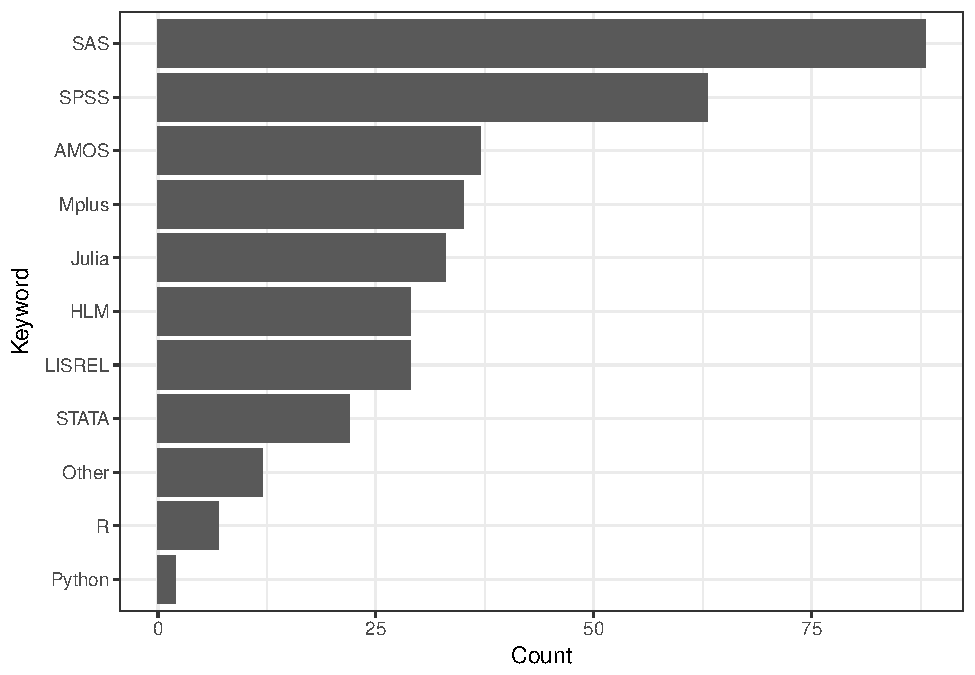
\includegraphics{aera_proposal_files/figure-latex/count-software-1.pdf}
\caption{\label{fig:count-software}Software count overall}
\end{figure}

When exploring the differences across the three journals in the current
sample, some notable differences appear (see Figure
\ref{fig:software-journal}). SAS, SPSS, LISREL, and Mplus are more
common in JEE compared to other software programs. EEPA is more likely
to use Python, Julia, or STATA and AERJ has a more consistent
distribution across the sofware programs.

\begin{figure}
\centering
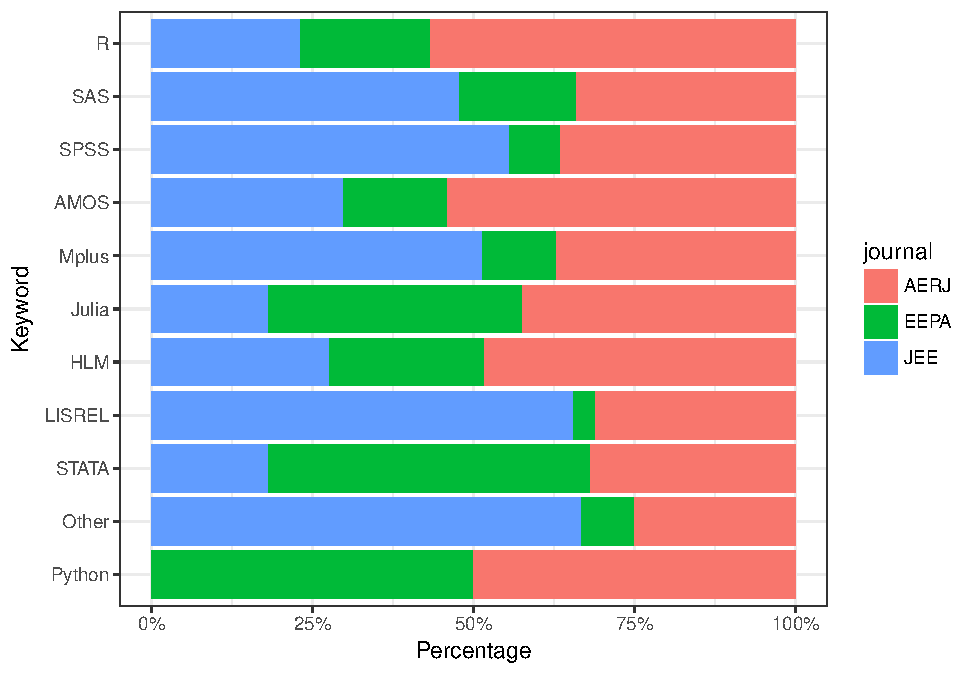
\includegraphics{aera_proposal_files/figure-latex/software-journal-1.pdf}
\caption{\label{fig:software-journal}Software counts by journal}
\end{figure}

Prior to AERA, more search terms, more journals, and gathering more
article meta data will be included in the research synthesis. These
additional data sources will allow a better understanding of the current
state of affairs in software usage, reproducible analysis, and software
citation/mention within educational journals.

\section{Scholarly Significance}\label{scholarly-significance}

Understanding the state of affairs in software usage in education is
important to help disentangle and highlight the importance of citing
statistical software and a reproducible research framework. Much more
attention has been given in other content areas such as biostatistics,
medicine, and psychology and the same standards should apply in
education. Recommendations will be given as to which information
regarding statistical software should accompany journal articles. This
study also aims to go a step further than others (see Muenchen, 2017) in
that the software usage will be explored with respect to journals and
also quantitative methodology. This will allow for a deeper exploration
of potential interactions between software usage and citations across
different journals and methodologies over time.

\section{References}\label{references}

\setlength{\parindent}{-0.5in} \setlength{\leftskip}{0.5in}

\hypertarget{refs}{}
\hypertarget{ref-rmarkdown}{}
Allaire, J., Cheng, J., Xie, Y., McPherson, J., Chang, W., Allen, J.,
\ldots{} Arslan, R. (2017). \emph{Rmarkdown: Dynamic documents for r}.
Retrieved from \url{https://CRAN.R-project.org/package=rmarkdown}

\hypertarget{ref-apa}{}
American Psychological Association. (2010). \emph{Publication manual of
the american psychological association}. Washington, D.C.: American
Psychological Association.

\hypertarget{ref-asendorpf2013}{}
Asendorpf, J. B., Conner, M., De Fruyt, F., De Houwer, J., Denissen, J.
J., Fiedler, K., \ldots{} others. (2013). Recommendations for increasing
replicability in psychology. \emph{European Journal of Personality},
\emph{27}(2), 108--119.

\hypertarget{ref-cooper2016}{}
Cooper, H. (2016). \emph{Research synthesis and meta-analysis: A
step-by-step approach} (Vol. 2). Sage publications.

\hypertarget{ref-ioannidis2014}{}
Ioannidis, J. P. (2014). How to make more published research true.
\emph{PLoS Medicine}, \emph{11}(10), e1001747.

\hypertarget{ref-iqbal2016}{}
Iqbal, S. A., Wallach, J. D., Khoury, M. J., Schully, S. D., \&
Ioannidis, J. P. (2016). Reproducible research practices and
transparency across the biomedical literature. \emph{PLoS Biology},
\emph{14}(1), e1002333.

\hypertarget{ref-pdfsearch}{}
LeBeau, B. (2016). \emph{pdfsearch: Search Tools for PDF Files}.
Retrieved from \url{https://github.com/lebebr01/pdfsearch}

\hypertarget{ref-muenchen}{}
Muenchen, R. A. (2017). The popularity of data science software.
Retrieved from \url{http://r4stats.com/articles/popularity/}

\hypertarget{ref-peng2009}{}
Peng, R. D. (2009). Reproducible research and biostatistics.
\emph{Biostatistics}, \emph{10}(3), 405--408.
doi:\href{https://doi.org/10.1093/biostatistics/kxp014}{10.1093/biostatistics/kxp014}

\hypertarget{ref-peng2011}{}
Peng, R. D. (2011). Reproducible research in computational science.
\emph{Science}, \emph{334}(6060), 1226--1227.

\hypertarget{ref-rpro}{}
R Core Team. (2017). \emph{R: A language and environment for statistical
computing}. Vienna, Austria: R Foundation for Statistical Computing.
Retrieved from \url{https://www.R-project.org/}

\hypertarget{ref-stodden2012}{}
Stodden, V. (2012). Reproducible research for scientific computing:
Tools and strategies for changing the culture. \emph{Computing in
Science \& Engineering}, \emph{14}(4), 13--17.

\hypertarget{ref-knitr}{}
Xie, Y. (2015). \emph{Dynamic documents with R and knitr} (2nd ed.).
Boca Raton, Florida: Chapman; Hall/CRC. Retrieved from
\url{http://yihui.name/knitr/}

\hypertarget{ref-knitrmanual}{}
Xie, Y. (2017). \emph{Knitr: A general-purpose package for dynamic
report generation in r}. Retrieved from \url{http://yihui.name/knitr/}






\end{document}
